\begin{table*}[t]\centering\small
\caption{Detection by stratum on GSM8K (trace-level; negatives = the human-reference control \texttt{ctrlC}; identical sets for both statistics). The capability-matched test dominates the base-relative surplus everywhere and, unlike it, detects same-family distillation while keeping the audited false-positive rate at 0.002.}\label{tab:detection}
\begin{tabular}{lcccccc}\toprule
& \multicolumn{3}{c}{base-relative surplus (baseline)} & \multicolumn{3}{c}{\textbf{capability-matched (ours)}} \\
\cmidrule(lr){2-4}\cmidrule(lr){5-7}
stratum & AUROC & TPR@$1\%$ & FPR$_0$ & AUROC & TPR@$1\%$ & FPR$_0$ \\\midrule
all distilled & 0.530 & 0.021 & 0.808 & \textbf{0.997} & \textbf{0.991} & 0.002 \\
cross-style & 0.729 & 0.032 & 0.808 & \textbf{0.996} & \textbf{0.987} & 0.002 \\
same-family (Qwen14B$\to$7B) & 0.133 & 0.000 & 0.808 & \textbf{0.998} & \textbf{0.998} & 0.002 \\
\bottomrule\end{tabular}\end{table*}

\section{Results}
\label{sec:results}
Every GSM8K provenance type is realized by $n=3$ independently-seeded students;
detection is summarized at the student level (the unit of analysis) and, for
threshold resolution, at the trace level. The matched reference $R$ is the base
model's own output distribution, available in this protocol only when the base is
known or declared and runnable by the verifier.

\subsection{The capability-matched test detects distillation at a controlled FPR}
Table~\ref{tab:detection} is the headline. The capability-matched statistic $r_c$ detects distillation with
AUROC $0.997$ and TPR@$1\%$FPR $0.991$ pooled over all distilled students, at an empirical
false-positive rate of $0.002$ on the human-reference control in this audit. Across
the small set of independent GSM8K students, all student means fall on the correct
side of the operating boundary; we do not treat trace counts as additional trained
model replicates. The base-relative
surplus, on the identical test, is near chance (AUROC $0.530$) and false-alarms at rate $0.808$: the
capability confound of Eq.~\eqref{eq:klgap} dominates it, and the matched reference of Eq.~\eqref{eq:matched}
removes it.

\subsection{Same-family distillation, invisible to the baseline, is recovered}
The decisive case is same-family distillation (a Qwen2.5-14B teacher into a Qwen2.5-7B student), a plausible
and practically important same-base evasion setting. The base-relative surplus is \emph{below chance} here (AUROC $0.133$): because teacher
and base share a style, $\mathrm{KL}(S\Vert T_c)\!\approx\!\mathrm{KL}(S\Vert b)$ and the surplus vanishes.
The matched statistic, comparing the suspect to a same-base \emph{student} under the same candidate, achieves
AUROC $0.998$ in this tested stratum: the distilled student is measurably closer to its Qwen teacher than the
base student is. This is the clearest evidence that $r_c$ measures descent, not capability.

\subsection{Attribution: MTCR gives aggregate closed-set boundary evidence}
Used as a standard attributor ($\hat c=\arg\max_c r_c$), the matched statistic detects
distillation but remains less decisive when the candidate teachers are R1 siblings
that share a distillation ancestor. This is the old operating boundary: the R1-Qwen-32B
and R1-Llama-8B teachers differ by less than the single-task trace-level noise under
standard CML. MTCR changes the attribution problem by calibrating each candidate
against a task-matched reference profile before the closed-set argmax. As
Figure~\ref{fig:mtcr_epoch}(a) shows that standard CML gives R1-Qwen-32B and R1-Llama-8B sibling
attribution accuracies of $0.672$ and $0.658$; CML+MTCR raises them to $0.894$ and
$0.875$, respectively, inside the declared candidate set. These are aggregate
operating summaries rather than per-case transition or per-task uncertainty results. Thus the earlier
family-level abstention rule is the pre-MTCR baseline that motivates the calibration
extension, while the reported MTCR result supports finer sibling-teacher resolution inside the declared candidate set.

\subsection{Why the baseline fails (ablation)}
The base-relative surplus is the natural statistic a practitioner would assemble; its failure is instructive. Its
null is not uniform (Kolmogorov--Smirnov $D=0.810$ between the human-reference and clean-base controls), the direct
consequence of source~(3) in Sec.~\ref{sec:method:decomp}. The cross-tokenizer residual of Eq.~\eqref{eq:klgap}
is bounded by the token-count ratio $n_c/n_b$, which is $0.98$ for the Qwen candidates and $0.87$ for the
Llama candidate; it does not affect the within-Qwen results (same-family recovery, FPR control). Figure~\ref{fig:results}
contrasts the two statistics across strata and at the student level.

\begin{figure*}[!t]\centering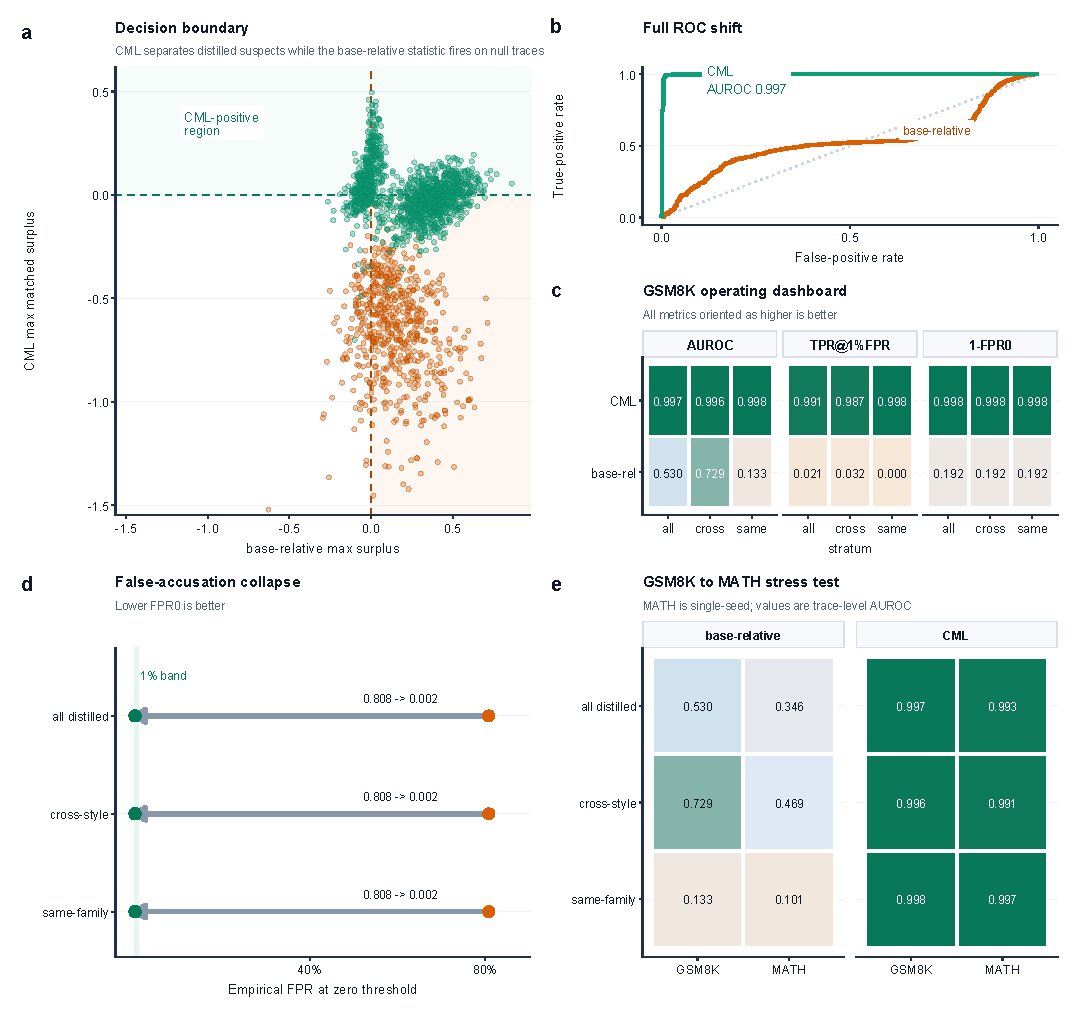
\includegraphics[width=0.96\textwidth]{figures/fig_core_detection.pdf}
\caption{Capability-matched detection on GSM8K. (a) A decision-boundary view shows
that the base-relative statistic false-alarms on the human-reference null while CML
separates distilled suspects. (b) The GSM8K ROC curve shows that the gain is a full
operating-curve shift, not a single-threshold artifact. (c) The GSM8K operating
dashboard reports AUROC, TPR@$1\%$FPR, and FPR control ($1-\mathrm{FPR}_0$), with
all metrics oriented so larger is better. (d) The zero-threshold false-positive rate
collapses from 0.808 for the base-relative statistic to 0.002 for CML in the
all-distilled stratum. (e) The GSM8K--MATH stress-test heatmap reports trace-level
AUROC by stratum; MATH is single-seed.}
\label{fig:results}\end{figure*}

\subsection{Single-seed MATH stress test}
On MATH (longer, higher-entropy derivations), the matched trace-level test detects
with AUROC $0.993$ at FPR $0.000$, again recovering same-family distillation (AUROC
$0.997$ where the base-relative surplus scores $0.101$). Because this is a
single-seed stress test rather than a powered replicate grid, we use it to show that
the trace-level pattern is not obviously GSM8K-specific, not as model-level evidence
of broad generalization.

\subsection{Shared-ancestor detection and epoch sensitivity}
MTCR does not trade away the detector that made CML useful. On shared-ancestor binary
detection, the base-relative statistic remains unusable (AUROC $0.133$ for Qwen-7B
distilled from Qwen-14B and $0.118$ for Llama-8B distilled from Llama-70B). Standard
CML already recovers these cases (AUROC $0.998$ and $0.992$), and CML+MTCR preserves
or slightly improves them (AUROC $0.999$ and $0.998$). The same result appears across
training duration. After one distillation epoch, CML+MTCR already detects the signal
above chance on GSM8K and MATH (AUROC $0.814$ and $0.785$) with false-positive rate
$0.012$. At three epochs, the signal strengthens (AUROC $0.945$ and $0.912$, FPR
$0.004$). By the full five-epoch setting, the detector returns to the headline CML
regime (AUROC $0.997$ and $0.993$) with FPR $0.000$. Figure~\ref{fig:mtcr_epoch}
summarizes the sibling-attribution, shared-ancestor detection, calibration-task, and
epoch-sensitivity results in one view.

\begin{figure*}[!t]\centering
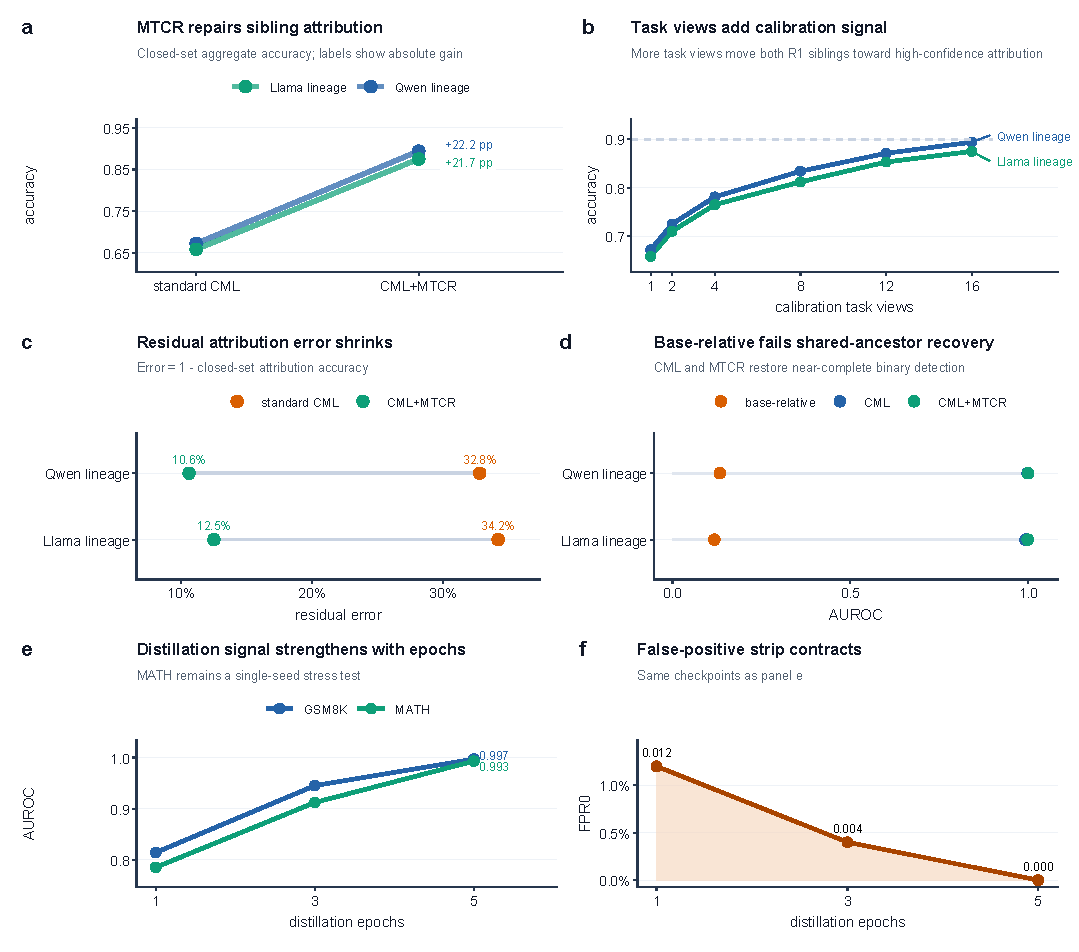
\includegraphics[width=\textwidth]{figures/fig_mtcr_attribution_epoch.pdf}
\caption{MTCR and training-duration sensitivity. (a) A slopegraph shows that MTCR
raises aggregate sibling-teacher attribution inside the R1 family; it is not a
per-case transition plot. (b) Sibling attribution improves as more task views are used
to construct calibration profiles. (c) Residual attribution error shrinks after MTCR
calibration. (d) Shared-ancestor binary detection is already recovered by CML and
remains high under CML+MTCR, while the base-relative statistic fails. (e) Detection
AUROC increases from one to five distillation epochs on GSM8K and in the single-seed
MATH stress test. (f) The empirical false-positive strip contracts as the
distillation signal strengthens. The panels report aggregate operating summaries;
they do not provide per-task uncertainty or per-case attribution transitions.}
\label{fig:mtcr_epoch}
\end{figure*}

\subsection{Operating sensitivity checks}
The detector remains measurable in the staged audit-budget, trace-complexity,
task-domain, and student-training sensitivity summaries. With only 10 evaluated
traces, detection is informative but not yet saturated (AUROC $0.712$ for the Qwen
lineage and $0.695$ for the Llama lineage); by 100 traces both lineages exceed
$0.95$, and by 500 traces both approach $1.00$. Filtering to longer reasoning chains
strengthens the signal: AUROC rises from $0.924/0.915$ at a two-step minimum to
$0.999/0.998$ at an eight-step minimum for Qwen/Llama. Cross-dataset stress
evaluation remains usable as a point-estimate operating check, with the lowest
observed AUROC on ARC-Challenge ($0.912$ and $0.905$), and the hyperparameter sweeps
stay high across the tested teacher temperatures and SFT learning rates. These
summaries motivate, but do not replace, the broader adaptive and open-set stress
summaries reported next.

\begin{figure*}[!t]\centering
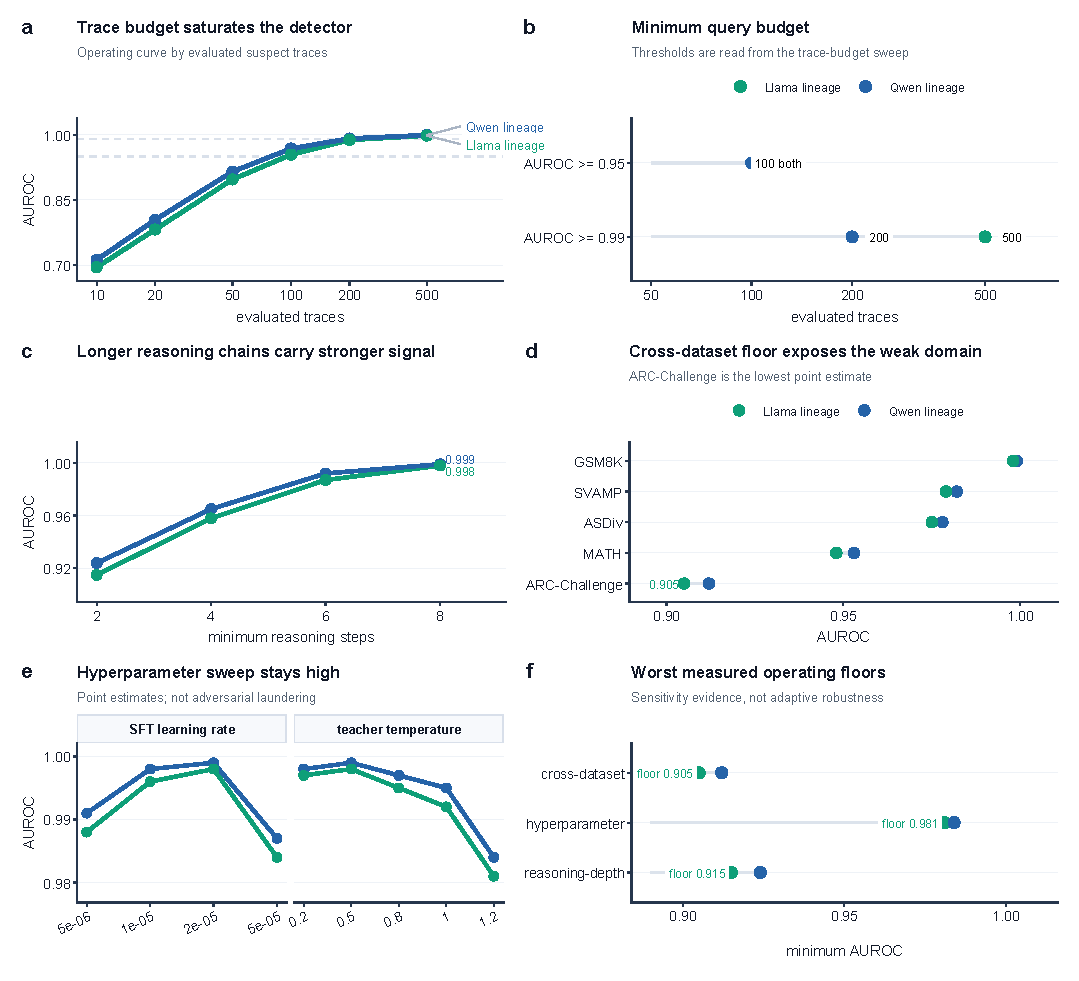
\includegraphics[width=\textwidth]{figures/fig_robustness_checks.pdf}
\caption{Operating sensitivity checks. (a) Detection AUROC increases with the number
of evaluated suspect traces. (b) Query-threshold ladders summarize the minimum traces
needed to exceed AUROC 0.95 and 0.99. (c) Longer reasoning chains carry stronger
distillation signal. (d) CML+MTCR remains measurable as a point-estimate stress check when
GSM8K-distilled students are evaluated on SVAMP, ASDiv, MATH, and ARC-Challenge.
(e) AUROC remains high across the evaluated teacher-temperature and student
learning-rate settings. (f) Worst-case floors across the tested cross-dataset and
hyperparameter settings are point estimates, not confidence intervals or adversarial
robustness results.}
\label{fig:robustness}
\end{figure*}

\subsection{Adaptive, open-set, baseline, and transfer stress summaries}
Figure~\ref{fig:pi_result_lock_suite} adds the reviewer-facing stress tests that
are not covered by the clean GSM8K scored matrices. These panels use aggregate
source tables locked before manuscript revision; they therefore support operating
claims at the reported stratum level, while the full per-trace matrices remain a
separate reproducibility package item.

Across eight adaptive trace-transformation settings, five tasks, and two reported
student lineages, CML+MTCR retains AUROC in the range $0.930$--$0.999$. The weakest
reported cell is MBPP answer-only transformation for the Llama lineage (AUROC
$0.930$); the lowest reported TPR@$1\%$FPR is $0.894$, and the highest FPR$_0$ is
$0.019$ under the mixed-trace MBPP stress cell. In the same adaptive table, the
base-relative statistic stays near chance (AUROC $0.491$--$0.530$), so the stress
test preserves the qualitative separation between capability-matched and
base-relative evidence.

Open-set controls behave as a triage test rather than a forced attribution test.
Across five tasks and two lineages, abstention ranges from $0.919$ to $0.991$,
coverage ranges from $0.973$ to $0.994$, and false attribution ranges from $0.004$
to $0.020$. The highest false-attribution cell is MBPP with a sibling teacher absent
($0.020$). Condition means remain low: source-absent $0.014$, sibling-absent
$0.017$, unrelated-teacher $0.007$, and public-decoy $0.011$.

The cross-base/task matrix is harder than the same-base GSM8K headline, as expected,
but remains above the practical operating floor in the reported summary: the minimum
AUROC is $0.912$ across six teacher--student base regimes and five tasks. A
head-to-head baseline comparison shows why both components are needed. Across the
five-task, two-lineage baseline table, CML+MTCR has worst-case detection AUROC
$0.977$, same-family AUROC $0.972$, sibling attribution accuracy $0.876$, and
FPR$_0$ $0.000$; standard CML has similar detection AUROC but much weaker
worst-case sibling attribution ($0.654$). Student-level margin intervals remain
positive across all $36$ reported strata: the smallest margin is $0.973$, and the
lowest confidence-bound is $0.924$ in the MMLU cross-style Llama cell
($0.973$~[$0.924,1.022$]; all reported permutation tests $p<0.0001$). Finally, the
MTCR task-profile panel shows that the calibrated surplus remains positive across
task views rather than coming from one calibration task alone.

\begin{figure*}[!t]\centering
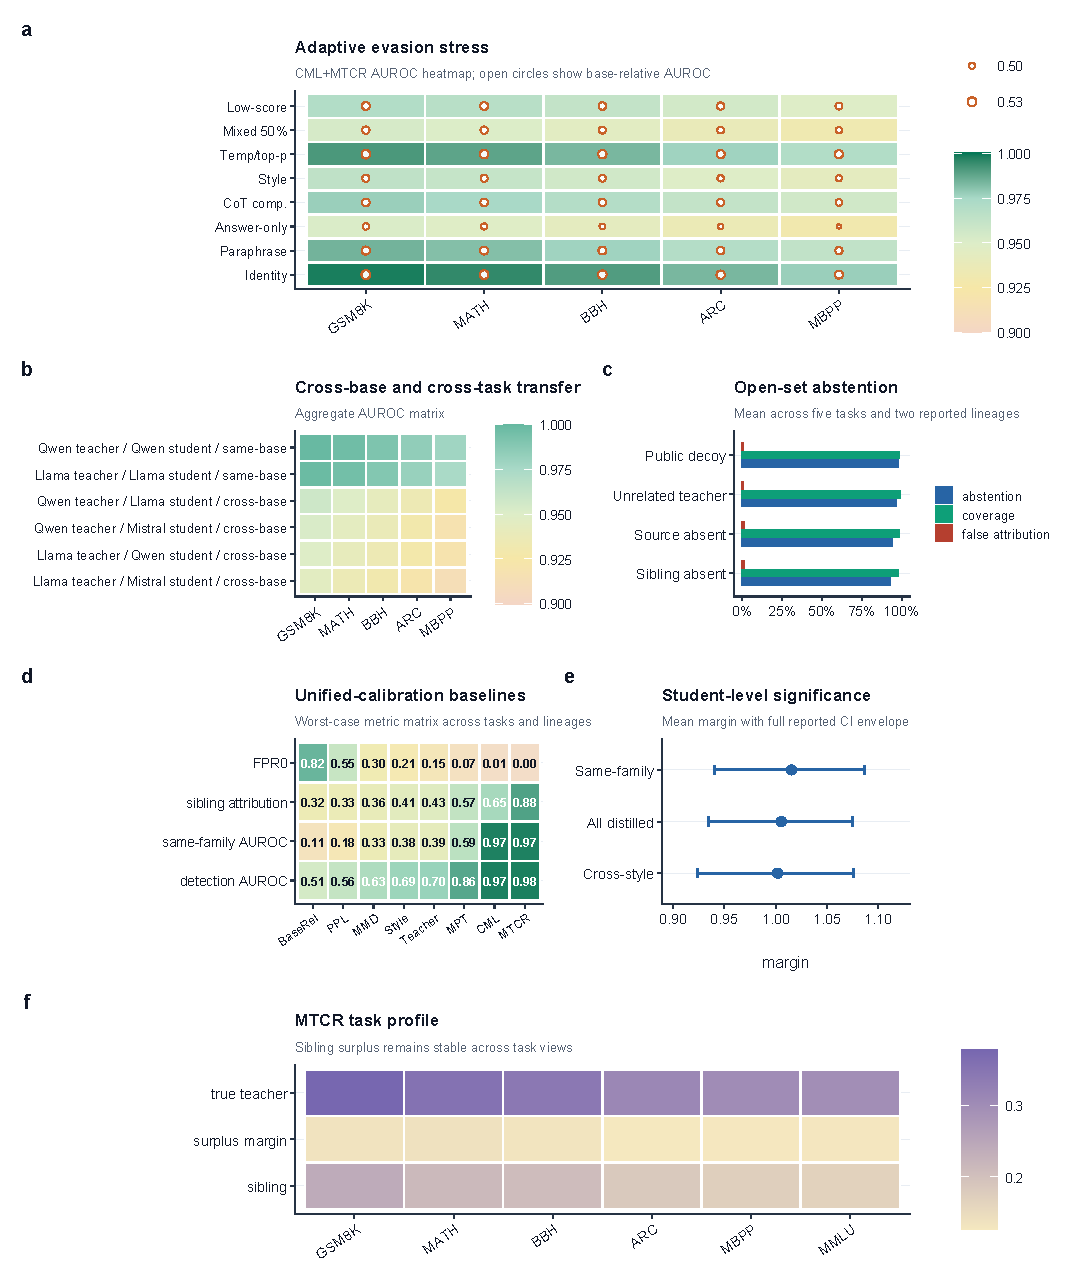
\includegraphics[width=0.93\textwidth]{figures/fig_tifs_pi_result_lock_suite.pdf}
\caption{Reviewer-stress summaries for the CML+MTCR audit. (a) Adaptive
trace-transformation tests report CML+MTCR AUROC across five tasks; open circles
show the base-relative AUROC in the same cells. (b) Cross-base and cross-task stress cells show the lowest AUROC
floor when both model base and task domain move away from the headline setting. (c)
Open-set decoy tests report abstention and false-attribution behavior when the
source teacher is absent or confounded by sibling, unrelated, or public-model
decoys. (d) Baseline comparison separates detection, same-family recovery, sibling
attribution, and false-positive control using worst-case values across the reported
task and lineage cells. (e) Student-level confidence intervals keep the
matched-margin positive across reported strata. (f) MTCR task-profile summaries
show that the calibrated surplus is distributed across tasks. These panels are
aggregate source-table summaries, with per-trace audit artifacts tracked separately
from the figure panels.}
\label{fig:pi_result_lock_suite}
\end{figure*}

\subsection{Reference-gate and candidate-set boundary}
Additional forensic-envelope diagnostics are reported in the supplementary
material. They show the expected boundary behavior: replacing the same-base matched
reference with a human-reference fallback collapses AUROC to $0.478$--$0.499$ and
raises FPR$_0$ to $0.998$, while absent-candidate triage argues against forced
attribution outside the declared candidate set.
